\newcommand{\pwidth}{.95\textwidth}
\subsection{Rectifier}
The simulated output from the half-wave rectifier circuit is shown in
Figure~\ref{fig:halfwavePlotV}.  As is shown, the maximum input voltage
is~\SI{17.401}{\volt} (zero-to-peak), implying an RMS voltage
of~\SI{12.3}{\volt} --- just one tenth of a volt higher than the designed value.
%
\begin{figure}[H]
	\centering
	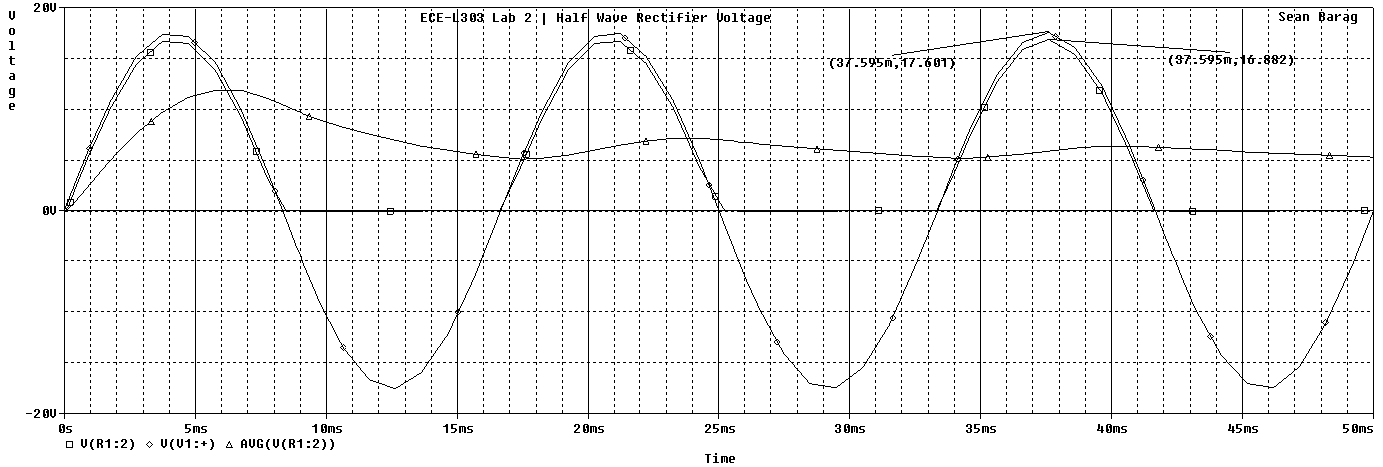
\includegraphics[width=\pwidth]{img/plot/halfwavePlot.PNG}
	\parbox{\pwidth}{
	\caption[PSpice Plot --- Half-wave Rectifier (Voltage)]{PSpice simulated
		input and output voltages as a function of time, as well as the average
		value of the output.  This data corresponds to the circuit in
		Figure~\ref{fig:schem1}.}
	\label{fig:halfwavePlotV}}
\end{figure}
%
Similarly, the output had a peak value of~\SI{16.648}{\volt} (zero-to-peak).
After dividing by~$\pi$, the average voltage was found to be~\SI{5.29}{\volt}
--- roughly~\SI{0.3}{\volt} lower than it should be.  The average value of the
output is also plotted on these axes.  As is expected, its value
approaches~\SI{5.29}{\volt} as more input cycles pass.  The decreased average
value is caused by the~\SI{0.7}{\volt} potential drop across the diode required
to turn it on, which is evident in the difference between the peak input and
output values.

An evaluation of power dissipation was also conducted, to ensure that certain
parts would be safe to use.  A plot of power dissipation over time is shown in
Figure~\ref{fig:halfwavePlotW}.
%
\begin{figure}[H]
	\centering
	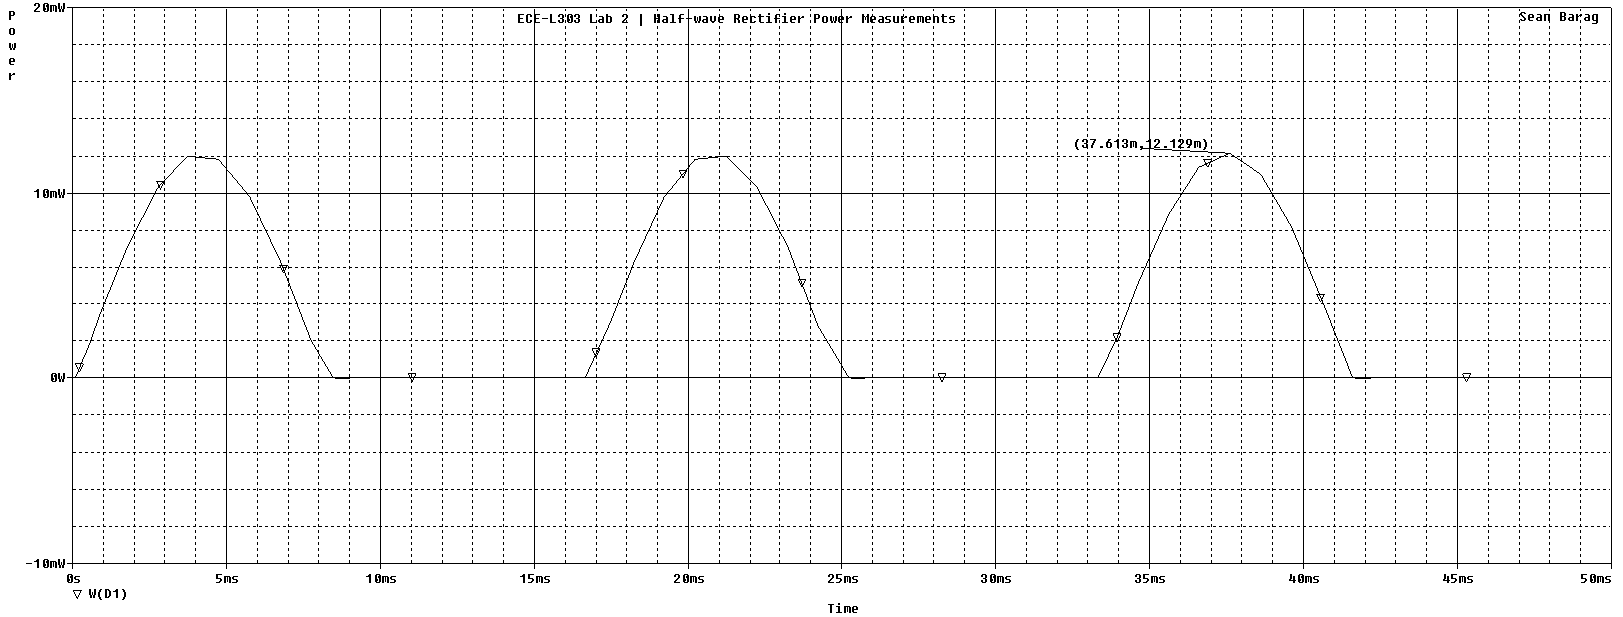
\includegraphics[width=\pwidth]{img/plot/halfwavePowerPlot.PNG}
	\parbox{\pwidth}{
	\caption[PSpice Plot --- Half-wave Rectifier (Power)]{Simulated power
		dissipation for the half-wave rectifier's diode shown in
		Figure~\ref{fig:schem1}.}
	\label{fig:halfwavePlotW}}
\end{figure}
%
The maximum power dissipated by the diode is shown as~\SI{12.129}{\milli\watt}.
Any diode with a maximum power dissipation of even one-eighth of a Watt will be
more than sufficient for this circuit.

\subsection{Voltage Regulator}
The regulated output of the zener diode-based regulator, as simulated by
PSpice, is plotted in Figure~\ref{fig:zenerPlotV}.  As is shown, the diode
begins to regulate the voltage when the input is\SI{10.085}{\volt}.
%
\begin{figure}[H]
	\centering
	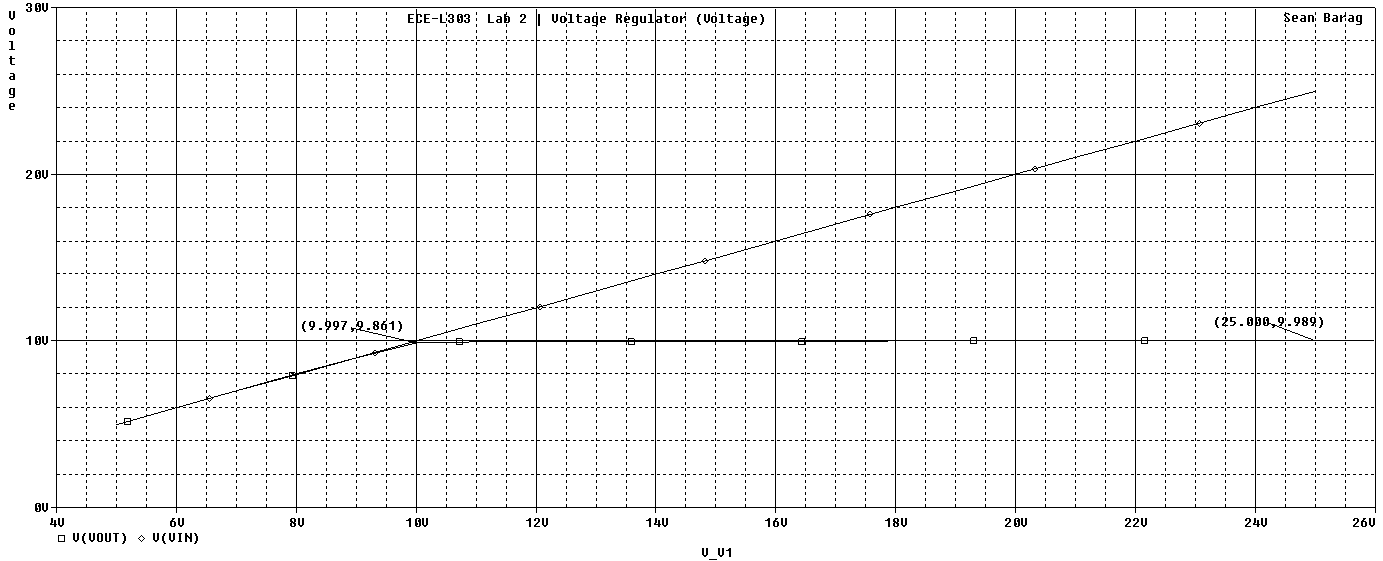
\includegraphics[width=\pwidth]{img/plot/zenerPlot.PNG}
	\parbox{\pwidth}{
	\caption[PSpice Plot --- Voltage Regulator (Voltage)]{Plot of simulated
	voltage regulator output for the circuit shown in Figure~\ref{fig:schem3}.
	The output is clearly regulated for all inputs above~$\sim$\SI{10}{\volt}.}
	\label{fig:zenerPlotV}}
\end{figure}
%
While regulated, the output voltage remains near the designed value of
~\SI{10}{\volt} DC, but tends to increase slightly due to a decrease in
efficiency in the diode as it heats up.  Where regulation begins, the output
measures~\SI{9.86}{\volt}, a value that increases to just~\SI{9.98}{\volt}
where the input voltage is~\SI{25}{\volt}.  This implies an increase of
just~\SI{8}{\milli\volt\per\volt}.

A power dissipation analysis was conducted for the zener diode circuit, as was
conducted with the half-wave rectifier.  Using PSpice's power probe, a plot of
the power dissipated by both the resistor and the zener diode was created.
This plot is reproduced below in Figure~\ref{fig:zenerPlotW}.
%
\begin{figure}[H]
	\centering
	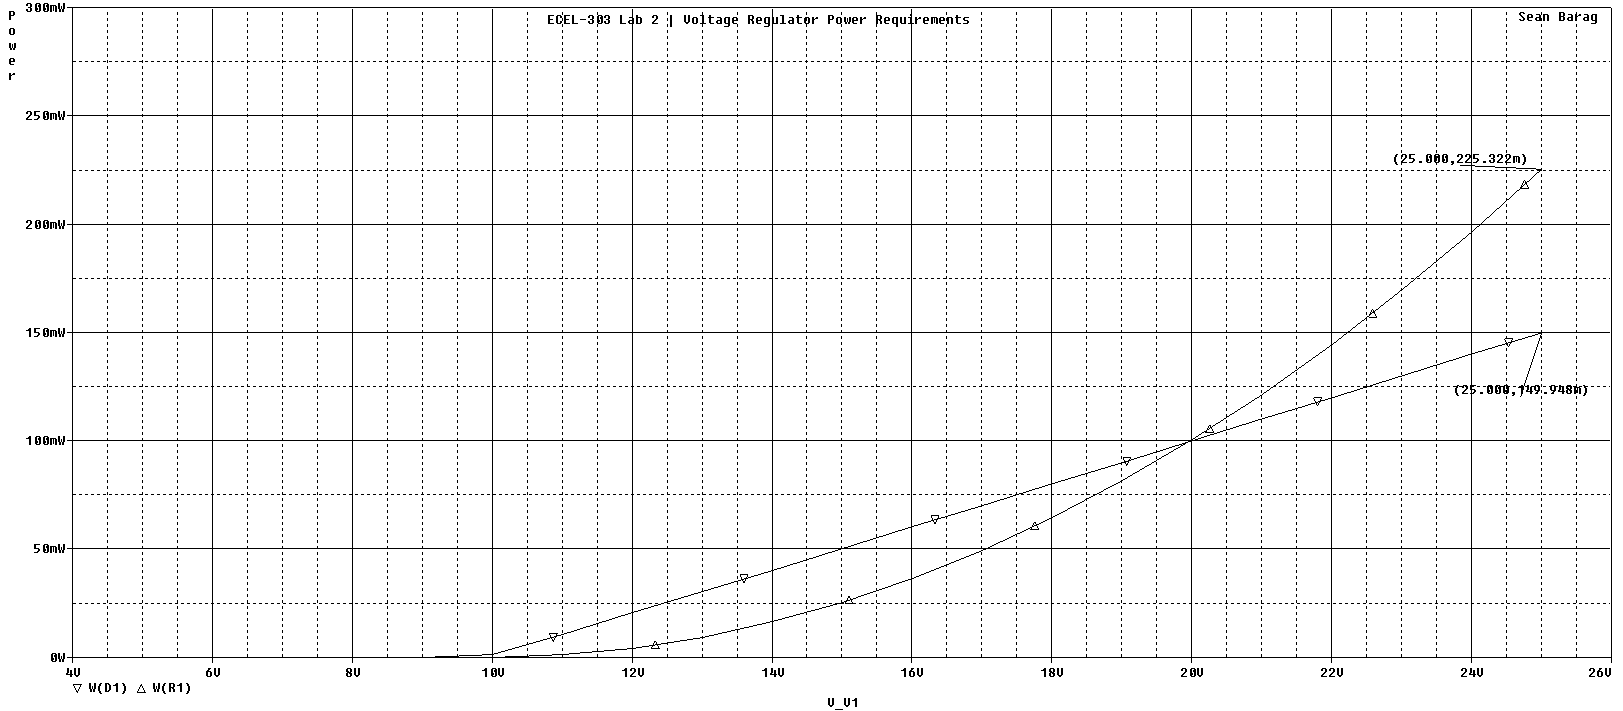
\includegraphics[width=\pwidth]{img/plot/zenerPowerPlot.PNG}
	\parbox{\pwidth}{
	\caption[PSpice Plot --- Voltage Regulator (Power)]{Simulated voltage
		regulator power dissipation for both the resistor and zener diode.
		This result shows that a quarter-watt resistor and diode are both
		sufficient for the tested circuit.}
	\label{fig:zenerPlotW}}
\end{figure}
%
According to the plot and PSpice's associated data, the maximum amount of power
dissipation required for the zener diode to be used safely
is~\SI{150}{\milli\watt}.  As such, a diode with maximum power rating of just a
quarter-watt can be safely used for this experiment.  Since the power
dissipated through the zener diode increases linearly, it can also be used for
input values up to and above~\SI{30}{\volt}.

The maximum value power dissipated through the resistor
is~\SI{225}{\milli\watt}, implying that a standard~\SI{1/4}{\watt} resistor
will be sufficiently capable for the range of inputs simulated here.  It should
be noted however that the power dissipated by the resistor follows a quadratic
increase, as is expected by the fact that power dissipated by an element is
simply the product of its resistance and the square of the current flowing
through it.  Since the resistance is constant and the current through the
device increases linearly according to Ohm's Law, it makes intuitive sense for
the power to increase quadratically.  As a result, it is not advised that a
quarter-Watt resistor be used for this experiment if the maximum input voltage
will be larger than~\SI{25}{\volt}.

\subsection{Constant Current Source}
PSpice was used to simulate two different constant current sources: one driven
by a~\SI{16}{\volt} source and one driven by a~\SI{32}{\volt} source.  The
resulting output voltage where the voltage source measures~\SI{16}{\volt} is
shown in Figure~\ref{fig:ccPlot16}.
%
\begin{figure}[H]
	\centering
	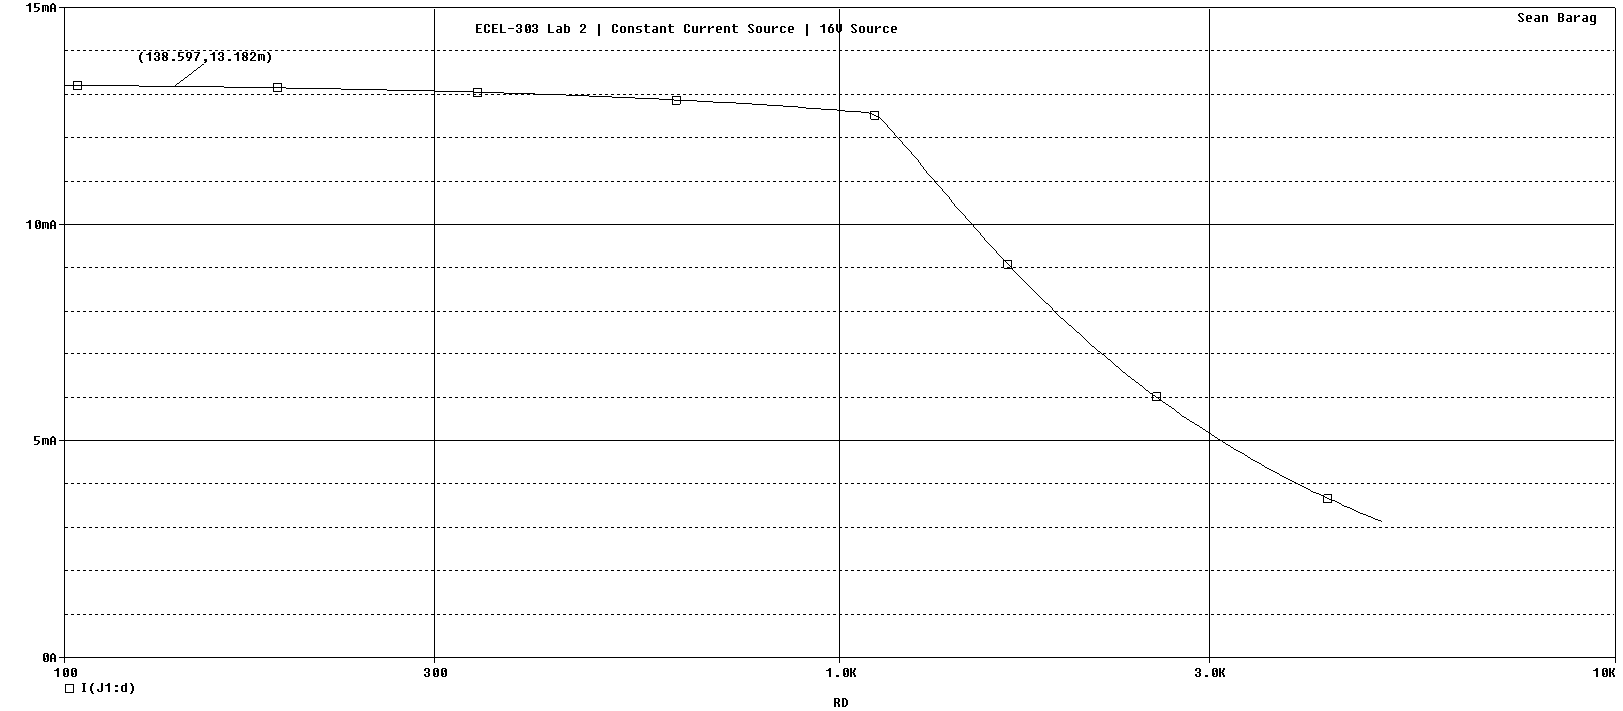
\includegraphics[width=\pwidth]{img/plot/constantCurrent16Plot.PNG}
	\parbox{\pwidth}{
	\caption[PSpice Plot --- Constant Current Source (\SI{16}{\volt})]{Constant
		current source simulation results for the case of a~\SI{16}{\volt}
		source, showing the affects of load resistance on output current.  Note
		the low threshold resistance compared to the counterpart simulation in
		Figure~\ref{fig:ccPlot32}.}
	\label{fig:ccPlot16}}
\end{figure}
%
By JFET used in this simulation is capable of regulating the current through
its drain util the drain resistance reaches roughly~\SI{1.15}{\kilo\ohm}.  For
loads above this value, the output current begins to decrease at a rate
of~\SI{0.002}{\milli\ampere\per\kilo\ohm}.

A similar effect occurred with the~\SI{32}{\volt} version of this circuit,
shown in Figure~\ref{fig:ccPlot32}.  Once the load resistance crosses a
threshold, the JFET begins to steadily lose its ability to regulate the current
flowing through the drain.
%
\begin{figure}[H]
	\centering
	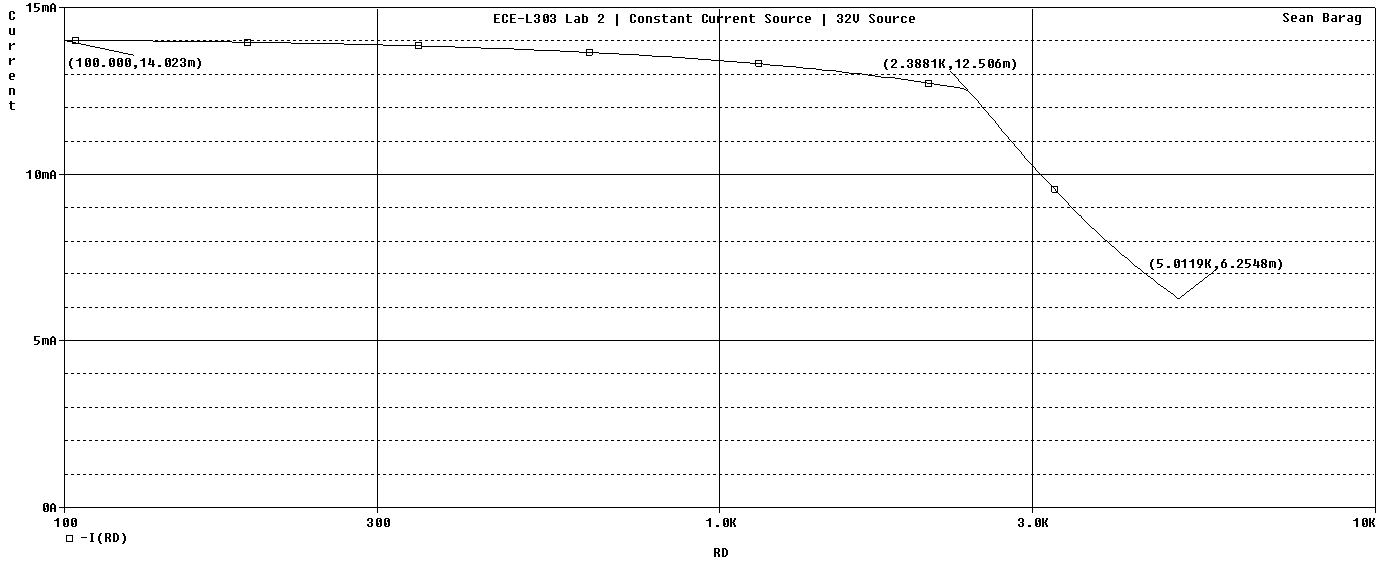
\includegraphics[width=\pwidth]{img/plot/constantCurrent32Plot.PNG}
	\parbox{\pwidth}{
	\caption[PSpice Plot --- Constant Current Source
		(\SI{32}{\volt})]{Simulated affects of load resistance on the output
		current for the constant current source shown in
		Figure~\ref{fig:schem4}, where the voltage source
		measures~\SI{32}{\volt}.  Note that the current begins decreasing at a
		higher resistance than its companion simulation in
		Figure~\ref{fig:ccPlot16}.}
	\label{fig:ccPlot32}}
\end{figure}
%
Compared to the~\SI{16}{\volt} source, this simulation shows a threshold
resistance of~\SI{2.4}{\kilo\ohm}.  For all greater resistances, the current
through the drain decreases at roughly~\SI{2.4}{\milli\ampere\per\kilo\ohm}.

\subsection{High Input Resistance Buffer Amplifier}
The high input resistance buffer amplifier was tested by monitoring the output
(the voltage across the emitter resistor) as the input voltage varied.  The
expected output is exactly one volt lower than the input voltage for any given
input.  PSpice's simulation data is plotted in Figure~\ref{fig:bjtPlotV}.
%
\begin{figure}[H]
	\centering
	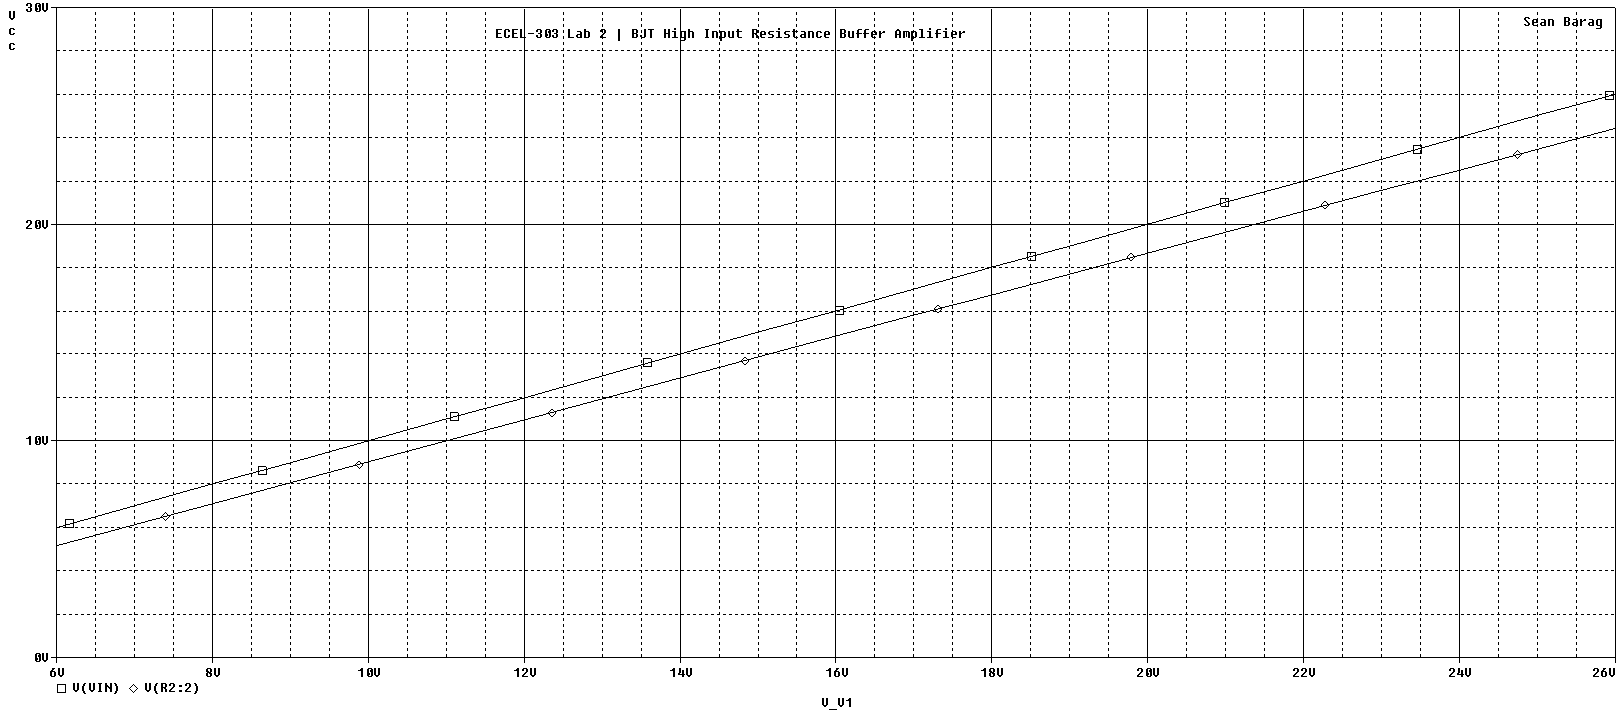
\includegraphics[width=\pwidth]{img/plot/bjtPlotV.PNG}
	\parbox{\pwidth}{
	\caption[PSpice Plot --- Buffer Amplifier (Voltage)]{Simulated output for
		the BJT high input resistance buffer amplifier, or ``emitter follower''
		amplifier.  Note the strong similarity between the input and output
		signals.}
	\label{fig:bjtPlotV}}
\end{figure}
%
Clearly, the output voltage closely mimics the input, thus justifying this
circuit's alternate name of ``emitter follower'' amplifier.  There is a bit of
a discrepancy, however; while the input grows at~\SI{1}{\volt\per\volt} as is
expected, the output grows at a rate of~\SI{0.96}{\volt\per\volt}.  This slight
difference means that such a configuration is not useful for high-voltage
inputs, as there will be a comparatively large discrepancy between input and
output in such a use.

When initially presenting the high input resistance buffer amplifier, the
student was given a requirement that the input impedance must never drop
below~\SI{320}{\kilo\ohm}.  TO ensure that this did not happen, the input
impedance was plotted by dividing the input voltage by the current through the
base resistor\footnote{This quotient was negated as a result of an assumption
PSpice makes, and should be treated as a workaround to a known quirk.}.  A plot
of the input resistance versus the input voltage, generated by PSpice, is shown
in Figure~\ref{fig:bjtPlotR}.
%
\begin{figure}[H]
	\centering
	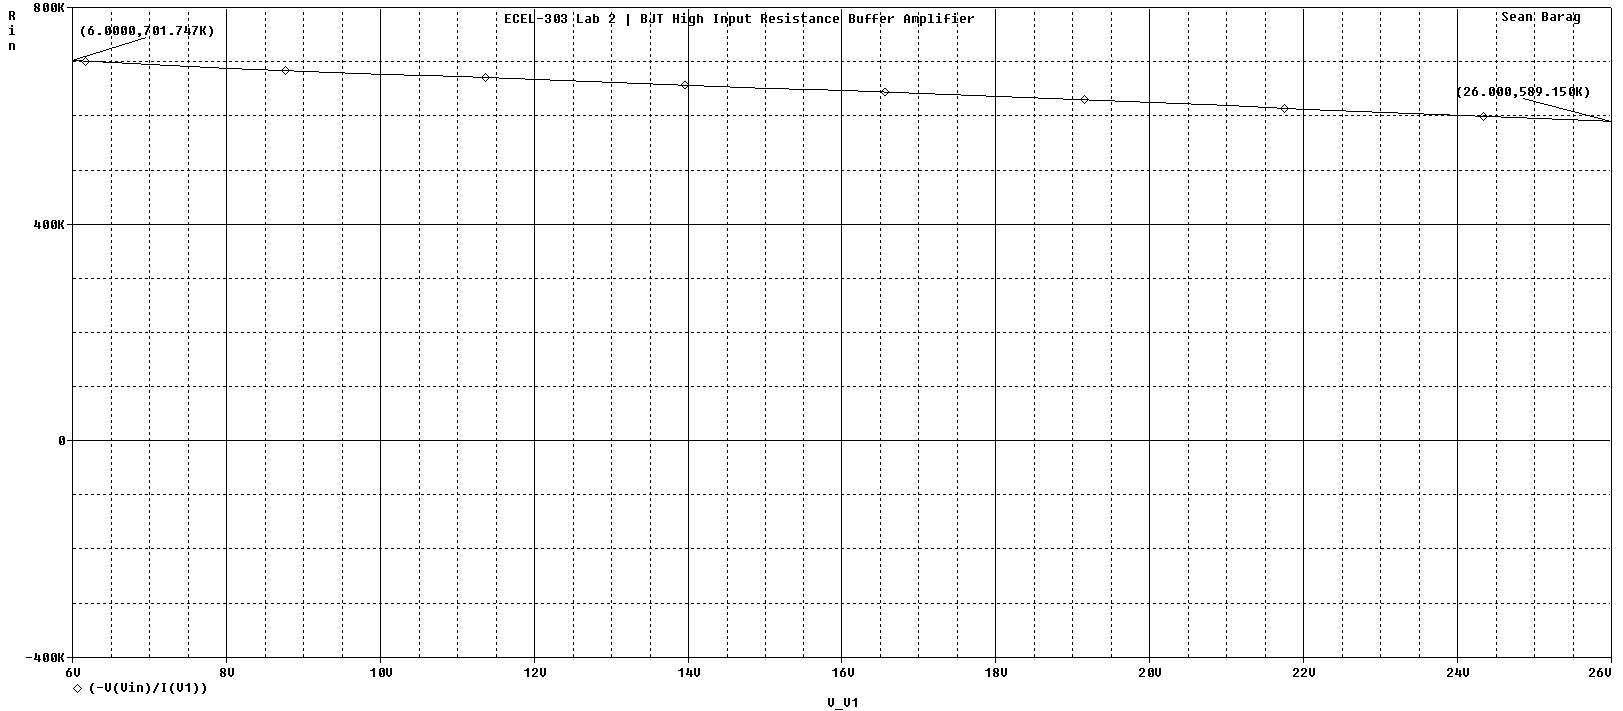
\includegraphics[width=\pwidth]{img/plot/bjtPlotR.PNG}
	\parbox{\pwidth}{
	\caption[PSpice Plot --- Buffer Amplifier (Resistance)]{Plot of the
		simulated input resistance, and how it changes with the input voltage.
		At no point does it dip below the specified minimum value
		of~\SI{320}{\kilo\ohm}.}
	\label{fig:bjtPlotR}}
\end{figure}
%
As is shown in the PSpice out, the input resistance is at its maximum when the
input is at its minimum, measuring roughly~\SI{700}{\kilo\ohm}.  The minimum
input resistance occurs at the maximum input voltage, resulting in an input
impedance of~\SI{590}{\kilo\ohm}.  While this resistor configuration will
satisfy all design constraints for the current range of inputs, inputs larger
than~\SI{26}{\volt} should signal the user to carefully monitor the input
resistance to ensure it does not dip below the required~\SI{320}{\kilo\ohm}
minimum.


